\chapter*{Введение}                         % Заголовок
\addcontentsline{toc}{chapter}{Введение}    % Добавляем его в оглавление

\paragraph*{Актуальность темы.}

\paragraph*{Цель работы.}

\paragraph*{Задачи работы.}

\paragraph*{Научная новизна работы.}

\paragraph*{Теоретическая и практическая значимость работы.}

\paragraph*{Положения выносимые на защиту.}
\begin{enumerate}
    \item \statementOneRU
    \item \statementTwoRU 
\end{enumerate}

\paragraph*{Апробация работы.}

\paragraph*{Достоверность научных достижений.}

\paragraph*{Внедрение результатов работы.}

\paragraph*{Публикации.} Список всех публикаций автора по теме диссертации:
\begin{refsection}[biblio/own.bib]
\nocite{*}
\printbibliography[
    keyword=own,
    %title={Список всех публикаций автора по теме диссертации}, 
    %heading=subbibliography,
    heading=none,
    resetnumbers=true
]
\end{refsection}



\paragraph*{Структура и объем диссертации. }
Диссертация состоит из~введения,
\formbytotal{totalchapter}{глав}{ы}{}{},
заключения и
\formbytotal{totalappendix}{приложен}{ия}{ий}{}.
%% на случай ошибок оставляю исходный кусок на месте, закомментированным
%Полный объём диссертации составляет  \ref*{TotPages}~страницу
%с~\totalfigures{}~рисунками и~\totaltables{}~таблицами. Список литературы
%содержит \total{citenum}~наименований.
%
Полный объём диссертации составляет
\formbytotal{TotPages}{страниц}{у}{ы}{}, включая
\formbytotal{totalcount@figure}{рисун}{ок}{ка}{ков} и
\formbytotal{totalcount@table}{таблиц}{у}{ы}{}.
Список литературы содержит
\formbytotal{citenum}{наименован}{ие}{ия}{ий}.


\begin{figure}
    \centering
    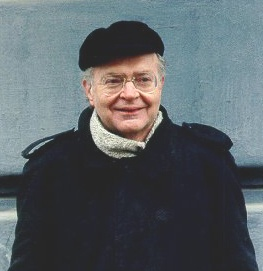
\includegraphics[width=0.6\linewidth]{images/knuth}
    \caption{Knuth}
    \label{fig:my_label}
\end{figure}